\documentclass[12pt]{article}
\usepackage[utf8]{inputenc}
\usepackage[spanish]{babel}
\usepackage{graphicx}
\usepackage{float}
\usepackage{hyperref}
\usepackage{amsmath}
\usepackage{amssymb}
\usepackage[
    type={CC},
    modifier={by-nc-sa}, 
    version={3.0},
]{doclicense}
\usepackage{verbatim}

\title{Memoria Algoritmo A Estrella}
\author{Nerea Jiménez González\\ Yhondri Acosta Novas}
\date{Abril 2020}

\begin{document}

\maketitle
\begin{figure}[H]
    \centering
    
\includegraphics[width=1\textwidth]{3-2016-07-21-Marca UCM Monocromo Negro.png}
\end{figure}

\newpage
\tableofcontents
\listoffigures
\newpage

\section{Detalles de la implementación}
\subsection{Lenguaje utilizado}
Para la implementación, se utiliza el lenguaje JAVA.
\subsection{Procedimiento seguido para la implementación}
En un primer lugar, resolvemos el problema que se da en el enunciado de la práctica para poder utilizarlo de base.\\
Para la lectura del archivo, creamos una clase \textit{Reader}, en la cual implementamos la lectura de los archivos de entrada.\\
Para la construcción del árbol final, implementamos una clase \textit{Node}, cuyo constructor recibe un \textit{String}, que será el valor seleccionado tras aplicar el \textbf{ID3}, y otro nodo para seguir en una futura recursión.\\
En la clase \textit{ID3} es donde implentamos el algoritmo como tal. 

El método id3 recibe 2 parámetros: \textit{mData} que contiene los ejemplos de los atributos, y \textit{restoAttributos} que contiene los atributos sobre los que se va a iterar.\\
Lo primero que nos encontramos en el método son los casos base, es decir, los casos que al cumplirse terminan esa rama recursiva y “regresa” desde donde se ha realizado la llamada.
\begin{itemize}
    \item Caso base1: La lista restoAttributos está vacía, en este caso “regresamos”
    \item Caso base2: Todos los ejemplos de mData son del mismo signo, en este caso “regresamos
\end{itemize}
En caso de no cumplir ninguno de los casos base, seguimos. 
\begin{enumerate}
    \item Obtenemos el elemento que minimice el mérito, esto lo hacemos llamando al método \textit{getBestAttribute}. El método \textit{getBestAttribute} itera sobre cada uno de los atributos. Por cada atributo itera obteniendo el mérito y comparando quedándose en la variable \textit{bestAttribute} el atributo con mejor mérito. Una vez ha terminado de iterar sobre todos los atributos, devuelve el mejor atributo obtenido
    \item Obtenemos y guardamos en una lista (\textit{noRepeatedValues}) los atributos del mejor atributo elegido en el paso anterior
    \item En otra lista, filtramos el resto de atributos de la lista de atributos
    \item  En un map llamado \textit{partitionDataMaxValue}, guardamos las filas de los ejemplos del mejor atributo elegido en el paso 1. Creamos un map llamado\textit{ nodes} que contendrá los nodos del árbol. 
    \item Iteramos sobre los valores de la lista \textit{noRepeatedValues}. En este bucle hacemos la llamada recursiva que nos devolverá el subárbol (conjunto de nodos), de la rama de este atributo. El nodo devuelto en la llamada recursiva lo añadiremos al mapa Nodes creado en el punto 4
    \item Finalmente regresamos devolviendo el Nodo compuesto del mejor atributo y el el mapa nodes que contiene el resto de nodos elegidos en esa rama. 
\end{enumerate}
Siguiendo estos pasos conseguimos la recursividad completa del algoritmo

\subsection{Ampliaciones realizadas}
Para la explicación de la recursividad, vamos a utilizar el atributo \textbf{Temperatura} como si fuese el atributo mejor de la iteración.\\
Una vez hemos elegido el primer nodo, aplicamos la recursividad para calcular los  subárboles.\\
Calculamos los nuevos atributos a partir del nodo elegido siguiendo los siguientes pasos:
\begin{enumerate}
    \item En la variable \textit{bestAttribute} guardamos el valor de nodo atributo seleccionado, por ejemplo \textbf{Temperatura}
    \item A continuación filtramos para quedarnos con los atributos de que aún no han sido seleccionados, siguiendo el ejemplo serían \textbf{Humedad, Viento y Jugar} y los guardamos en una lista de strings llamada \textit{newRestoAttributos}
    \item Obtenemos los atributos del atributo elegido,  de \textbf{Temperatura} serían, caluroso, frío, templado y lo guardamos en un set de \textit{Strings} llamado, \textit{noRepeatedValue}s
    \item Iterando sobre \textit{noRepeatedValues}, dejamos en una lista llamada \textit{partition} los atributos restantes de todos los elementos de \textit{noRepeatedValues} excepto el mejor
\end{enumerate}

Finalmente, devolvemos el valor de id3(partition, newRestoAtrtributos).

\section{Código ejecutable}
Se adjunta en el archivo formato zip, con nombre \textbf{Código}.

\subsection{Simulación}
Al ejecutar p2.jar se abre la siguiente ventana.
\begin{figure}[H]
    \centering
    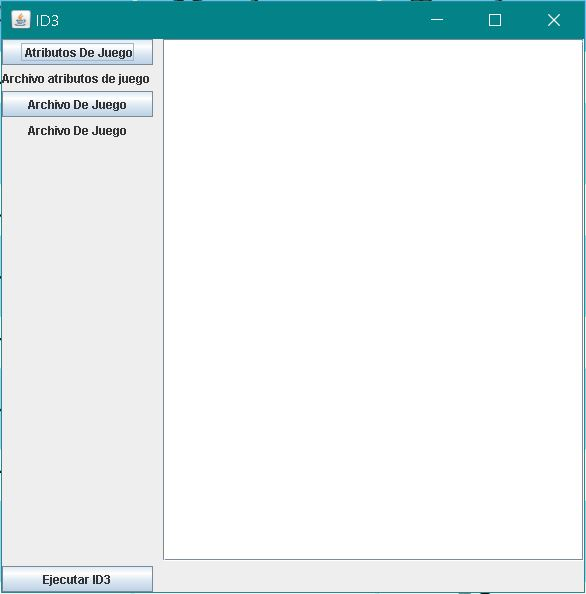
\includegraphics[width=0.75\textwidth]{ventana.JPG}
    \caption{Ventana inicial}
\end{figure}
Elegimos los archivos en los cuales está la información para poder ejecutar el algoritmo.
\begin{figure}[H]
    \centering
    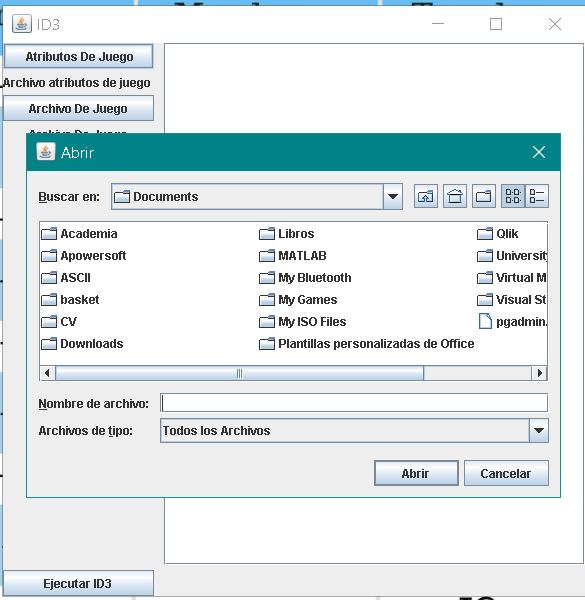
\includegraphics[width=0.75\textwidth]{click.JPG}
    \caption{Ventana elección de archivos}
\end{figure}
Tras elegir ambos archivos, clickeamos el botón de Ejecutar ID3 y en la parte derecha de la ventana podemos ver el resultado tras aplicar el algoritmo.\\
Hemos intentado recrear el árbol que se originaría:
\begin{itemize}
    \item -\textgreater : indica el atributo seleccionado
    \item = : indica el valor que toma el atributo seleccionado
\end{itemize}
Si no se llega a seleccionar el valor Jugar, significa que no disponemos de suficiente información para continuar por esa rama. 
\begin{figure}[H]
    \centering
    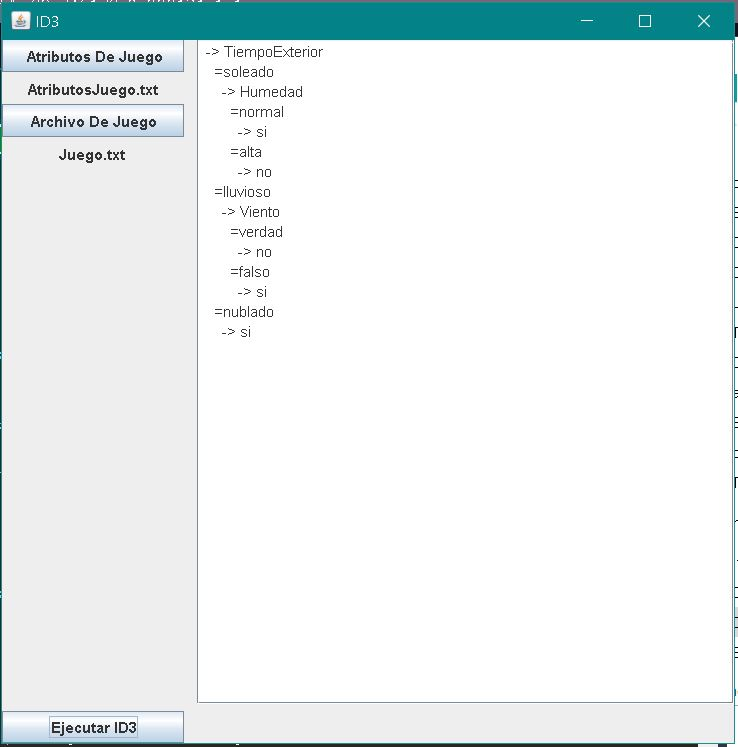
\includegraphics[width=0.75\textwidth]{final.JPG}
    \caption{Ventana final}
\end{figure}
En este ejemplo, el primer atributo seria \textbf{TiempoExterior}. Según sea el valor de este atributo:
\begin{itemize}
    \item \textbf{soleado:} en este caso no hemos acabado la recursión. El siguiente nodo en el árbol sería el atributo \textbf{Humedad}. Y con esta elección ya terminariamos esta rama.
    \item \textbf{lluvioso:} en este caso no hemos acabado la recursión. El siguiente nodo en el árbol sería el atributo \textbf{Viento}, y con esto terminariamos esta rama.
    \item \textbf{nublado:} siempre se juega si se tiene este valor.
\end{itemize}
De esta forma obtendriamos el árbol de decisión.

\section{Manual de usuario}
En el zip adjunto, hay un archivo ejecutable denominado \textbf{p2.jar}. Ejecutamos este archivo con doble click.\\
Una vez aparezca la venta, clickeamos en el botón \textit{Atributos de Juego} para seleccionar el archivo que contiene los atributos del Juego. Después, clickeamos en el segundo botón \textit{Archivo de Juego} para seleccionar el archivo de Juego.
\begin{figure}[H]
    \centering
    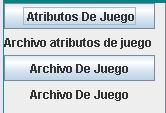
\includegraphics[width=0.25\textwidth]{Captura.JPG}
    \caption{Botón para selección de archivos}
\end{figure}
Una vez seleccionados ambos archivos, clickeamos el botón de la esquina inferior izquierda \textit{Ejecutar ID3}.
\begin{figure}[H]
    \centering
    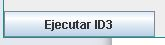
\includegraphics[width=0.25\textwidth]{2.JPG}
    \caption{Botón para ejecutar ID3}
\end{figure}
Tras clickear este botón, en la parte derecha de la ventana nos apareceran los atributos y sus valores elegidos en cada iteración, como hemos visto en el apartado de Simulación.
\newpage
\vspace*{\fill}
\begin{verbatim}
    Memoria Práctica 2
    Abril 2020
    Ult. actualización 29 de abril de 2020
\end{verbatim}
\LaTeX{} lic. LPPL \& Nerea Jiménez y Yhondri Acosta \& CC-ZERO
\doclicenseThis
\end{document}
